
%\documentclass[a4paper,11pt]{article}
\documentclass{article}

\usepackage[hangul]{kotex}
\usepackage{woosung_hw}
\usepackage{woosung_math}
\usepackage{mathtools}
\usepackage{stmaryrd}
\usepackage{float}
\usepackage{multirow}
\usepackage{array}

%\usepackage[bitstream-charter]{mathdesign}
%\usepackage[T1]{fontenc}

\setlength{\hoffset}{-25pt}
\addtolength{\textwidth}{50pt}
\setlength{\voffset}{-60pt}
\addtolength{\textheight}{130pt}

\newcommand{\w}[1]{\ensuremath{\textit{#1}}}
\newcommand{\x}{\times}
\newcommand{\rem}{\mtt{\%}}
\newcommand{\rar}{\rightarrow}
\newcommand{\Rar}{\Rightarrow}
\newcommand{\U}{\cup}
\newcommand{\join}{\sqcup}
\newcommand{\ttt}[1]{\texttt{#1}}
\newcommand{\mtt}[1]{\mathtt{#1}}
\newcommand{\bigspace}{\,\,\,\,\,\,\,\,}

\newcommand{\op}[2]{\mtt{#1(}#2\mtt{)}}
\newcommand{\module}[3]{\mtt{#1(}#2\mtt{)(}#3\mtt{)}}
\newcommand{\conc}{\mtt{@}}
\newcommand{\ind}[1]{\mtt{[}#1\mtt{]}}
\newcommand{\indr}[2]{\mtt{[}#1\mtt{:}#2\mtt{]}}
\newcommand{\ifs}[3]{\mtt{if}\,\,#1\,\,\mtt{then}\,\,#2\,\,\mtt{else}\,\,#3}

\newenvironment{prepost}[4]{
  \begin{tabular}{|>{\centering}m{0.4\textwidth}|p{0.6\textwidth}|}
    \hline
    \multicolumn{2}{|l|}{\texttt{#1}} \\ \hline
      \multirow{4}{*}{#2}
     & Require \\ \cline{2-2}
     & #3 \\ \cline{2-2}
     & Guarantees \\ \cline{2-2}
     & #4 \\ \hline
  \end{tabular}
}

\newenvironment{prepostc}[5]{
  \begin{tabular}{|>{\centering}m{0.4\textwidth}|p{0.6\textwidth}|}
    \hline
    \multicolumn{2}{|l|}{\texttt{#1}} \\ \hline
      \multirow{6}{*}{#2}
     & Require \\ \cline{2-2}
     & #3 \\ \cline{2-2}
     & Guarantees \\ \cline{2-2}
     & #4 \\ \cline{2-2}
     & Comment\\ \cline{2-2}
     & #5 \\ \hline
  \end{tabular}
}

\newenvironment{onlyc}[3]{
  \begin{tabular}{|>{\centering}m{0.4\textwidth}|p{0.6\textwidth}|}
    \hline
    \multicolumn{2}{|l|}{\texttt{#1}} \\ \hline
      \multirow{2}{*}{#2}
     & Comment\\ \cline{2-2}
     & #3 \\ \hline
  \end{tabular}
}

\newenvironment{itemizec}{
  \begin{itemize}
}{
  \end{itemize}
  \quad
  \vspace{-1em}
}


\begin{document}

\setlist{nolistsep}
\nointerlineskip
\par\noindent
\setlength{\parindent}{0pt}


\section*{Convolutional Layers}
\subsection*{\ttt{torch.nn.Conv2d}}%{{{
\prepostc{torch.nn.Conv2d(in, out, kernel\_size, stride=1, padding=0,
dilation=1, groups=1)(x)}{
  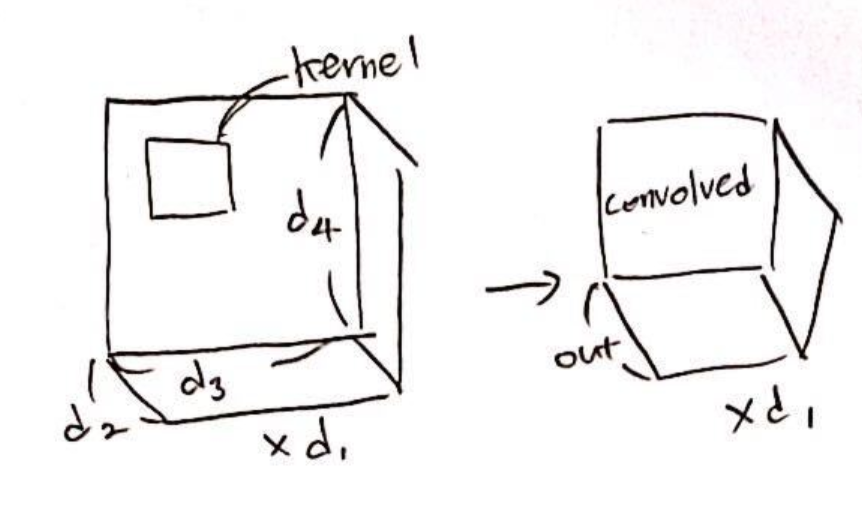
\includegraphics[height=12em]{resources/conv2d.png}
}{
  \begin{itemizec}
    \item $|x| = (d_1, d_2, d_3, d_4)$\bigspace ($rank = 4$)
    \item $d_2 = in$
    \item $kernel\_size[0] \leq d_3 + 2 \x padding[0]$
    \item $kernel\_size[1] \leq d_4 + 2 \x padding[1]$
    \item $groups | in$ and $groups | out$
  \end{itemizec}
}{
  \begin{itemizec}
    \item $|y| = (d_1, out, h, w)$ where.. refers to the proof tree.
  \end{itemizec}
}{
  \begin{itemizec}
    \item Convolution layer입니다. 선배님의 자료를 \ttt{pytorch}의 사용에 맞게
    풀어 쓴 것입니다.
    \item $kernel\_size$, $stride$와 같은 옵션은 튜플로 구성될 수도 있습니다.
    (가로 세로에 대한 필터크기가 서로 다르도록) 이 경우를 위하여 proof 트리에서
    $kernel\_size[0], [1]$과 같은 표기를 사용하였습니다. 튜플이 아니라 스칼라
    입력인 경우, $kernel\_size[0], [1]$은 모두 $kernel\_size$와 같습니다.
    \item 추가적인 옵션을 더하여 \ttt{Conv2d(in, out, k, s, p, d, g, bias=True,
    padding\_mode=`zeros')}로 사용하기도 하지만, 뒤의 두 \ttt{bias},
    \ttt{padding\_mode}는 출력 shape에 아무런 영향을 주지 않습니다.
  \end{itemizec}
}
\begin{align*}
  \frac
  {
    \begin{array}{l}
      \sigma \vdash E \Rar e, c \\
      h = \left\lfloor \frac{e[3] + 2 \x padding \ind{0} - dilation \ind{0}
        \x (kernel\_size \ind{0} - 1) - 1}{stride \ind{0}} \right\rfloor + 1 \\
      w = \left\lfloor \frac{e[4] + 2 \x padding \ind{1} - dilation \ind{1}
        \x (kernel\_size \ind{1} - 1) - 1}{stride \ind{1}} \right\rfloor + 1 \\
      e' = (e[1], out, h, w) \\
      c_{dim} = \{ (\op{rank}{e} = 4) \land (e[2] = in) \} \\
      c_h = \{ (kernel\_size\ind{0} \leq e[3] + 2 \x padding \ind{0}) \} \\
      c_w = \{ (kernel\_size\ind{1} \leq e[4] + 2 \x padding \ind{1}) \} \\
      c_{group} = \{ (in \rem groups = 0) \land (out \rem groups = 0) \}
    \end{array}
  }
  {
    \sigma \vdash \module{Conv2d}{in, out, kernel\_size, stride=1, padding=0,
      dilation=1, groups=1}{E} \Rar e', c \cup c_{dim} \cup c_h \cup c_w \cup
      c_{group}
  } \\
  \\
  \text{$kernel\_size, stride, padding, dilation$는 가로-세로별 2-tuple로도 들어갈
  수 있음} \\
  \text{이 경우를 위해 $stride\ind{0}, stride\ind{1}$으로 표기함} \\
  \text{만일 $stride$가 튜플이 아닌 스칼라라면 $stride\ind{0}$ 또는 $\ind{1}$은
    $stride$ 값 자체를 의미}
\end{align*}

\subsection*{(Builtins) \ttt{torch.conv2d}, \ttt{torch.nn.functional.conv2d}}
\prepostc{torch.conv2d(input, filter, bias=None, stride=1, padding=0,
dilation=1, groups=1)}{
  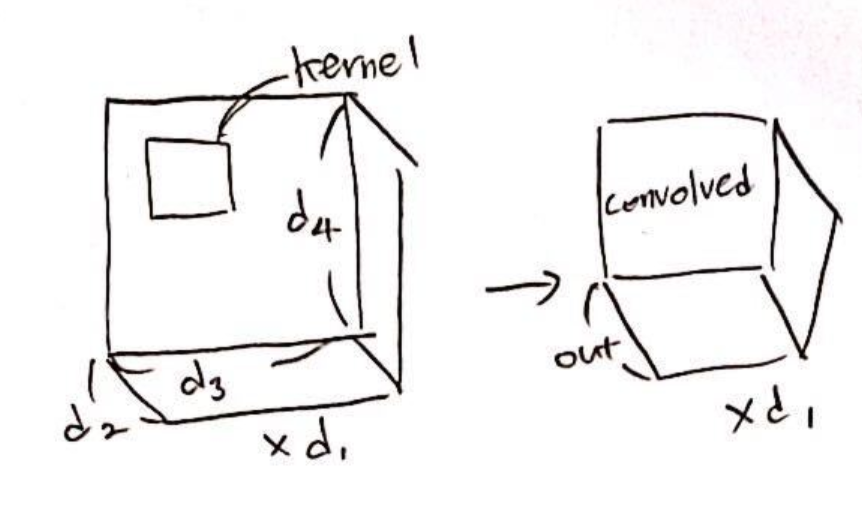
\includegraphics[height=12em]{resources/conv2d.png}
}{
  \begin{itemizec}
    \item $|input| = (batch, in, h_{in}, w_{in})$\bigspace ($rank = 4$)
    \item $|filter| = (out, in\_{group}, h_{filter}, w_{filter})$\bigspace
      ($rank = 4$)
    \item $bias$ is $None$ or $|bias| = (out)$
    \item $h_{filter} \leq h_{in} + 2 \x padding[0]$
    \item $w_{filter} \leq w_{in} + 2 \x padding[1]$
    \item $groups | in$, $groups | out$ and $in\_{group} \x group = in$
  \end{itemizec}
}{
  \begin{itemizec}
    \item $|y| = (batch, out, h, w)$ where.. refers to the proof tree.
  \end{itemizec}
}{
  \begin{itemizec}
    \item 컨볼루션 계산을 위해 사용하는 빌트인 함수입니다.
    \item \ttt{torch.conv2d}, \ttt{torch.nn.functional.conv2d} 모두 같은
    방식으로 작동됩니다.
  \end{itemizec}
}
\begin{align*}
  \frac
  {
    \begin{array}{l}
      \sigma \vdash E \Rar e, c \\
      \sigma \vdash F \Rar f, c \\
      \sigma \vdash B \Rar b, c \bigspace \text{if $B$ is not $None$} \\
      (batch, in, h_{in}, w_{in}) = e \\
      (out, in\_group, h_{filter}, w_{filter}) = f \\
      h = \left\lfloor \frac{h_{in} + 2 \x padding \ind{0} - dilation \ind{0}
        \x (h_{filter} - 1) - 1}{stride \ind{0}} \right\rfloor + 1 \\
      w = \left\lfloor \frac{w_{in} + 2 \x padding \ind{1} - dilation \ind{1}
        \x (w_{filter} - 1) - 1}{stride \ind{1}} \right\rfloor + 1 \\
      e' = (batch, out, h, w) \\
      c_{dim} = \{ (\op{rank}{e} = 4) \land (\op{rank}{f} = 4) \} \\
      c_{bias} = \{ ((B = None) \lor (\op{rank}{b} = 1 \land b[1] = out)) \} \\
      c_h = \{ (h_{filter} \leq h_{in} + 2 \x padding \ind{0}) \} \\
      c_w = \{ (w_{filter} \leq w_{in} + 2 \x padding \ind{1}) \} \\
      c_{group} = \{ (in \rem groups = 0) \land (out \rem groups = 0)
        \land (in\_group \x groups = in)\}
    \end{array}
  }
  {
    \sigma \vdash \op{conv2d}{E, F, B=None, stride=1, padding=0,
      dilation=1, groups=1} \Rar e', c \cup c_{dim} \cup c_{bias} \cup c_h \cup
      c_w \cup c_{group}
  } \\
  \\
  \text{$kernel\_size, stride, padding, dilation$는 가로-세로별 2-tuple로도 들어갈
  수 있음} \\
  \text{이 경우를 위해 $stride\ind{0}, stride\ind{1}$으로 표기함} \\
  \text{만일 $stride$가 튜플이 아닌 스칼라라면 $stride\ind{0}$ 또는 $\ind{1}$은
    $stride$ 값 자체를 의미}
\end{align*}%}}}

\subsection*{\ttt{torch.nn.Conv1d}}%{{{
\prepostc{torch.nn.Conv1d(in, out, kernel\_size, stride=1, padding=0,
dilation=1, groups=1)(x)}{
  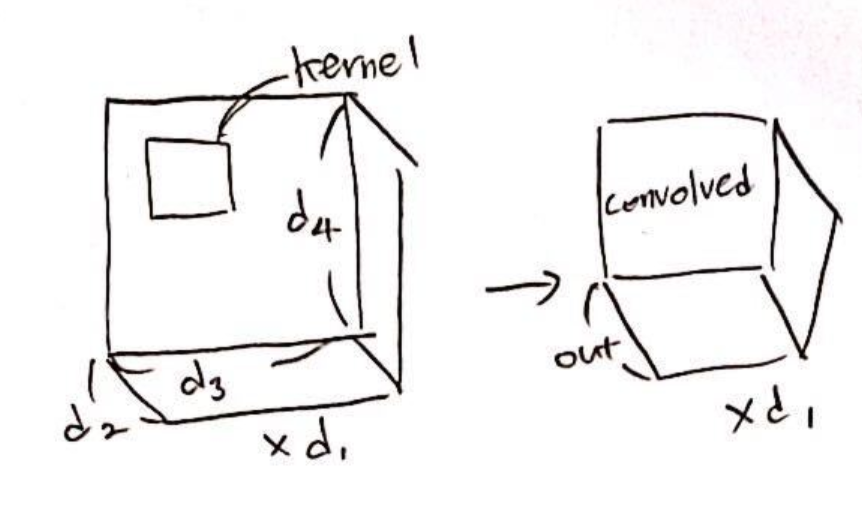
\includegraphics[height=12em]{resources/conv2d.png}
}{
  \begin{itemizec}
    \item $|x| = (d_1, d_2, d_3)$\bigspace ($rank = 3$)
    \item $d_2 = in$
    \item $kernel\_size \leq d_3 + 2 \x padding$
    \item $groups | in$ and $groups | out$
  \end{itemizec}
}{
  \begin{itemizec}
    \item $|y| = (d_1, out, w)$ where.. refers to the proof tree.
  \end{itemizec}
}{
  \begin{itemizec}
    \item Convolution 1차원 레이어입니다.
    \item $kernel\_size$, $stride$ 등은 1차원 튜플로 구성될 수도 있습니다.
    \item 추가적인 옵션을 더하여 \ttt{Conv1d(in, out, k, s, p, d, g, bias=True,
    padding\_mode=`zeros')}로 사용하기도 하지만, 뒤의 두 \ttt{bias},
    \ttt{padding\_mode}는 출력 shape에 아무런 영향을 주지 않습니다.
  \end{itemizec}
}
\begin{align*}
  \frac
  {
    \begin{array}{l}
      \sigma \vdash E \Rar e, c \\
      w = \left\lfloor \frac{e[3] + 2 \x padding  - dilation
        \x (kernel\_size - 1) - 1}{stride} \right\rfloor + 1 \\
      e' = (e[1], out, w) \\
      c_{dim} = \{ (\op{rank}{e} = 3) \land (e[2] = in) \} \\
      c_h = \{ (kernel\_size \leq e[3] + 2 \x padding) \} \\
      c_{group} = \{ (in \rem groups = 0) \land (out \rem groups = 0) \}
    \end{array}
  }
  {
    \sigma \vdash \module{Conv1d}{in, out, kernel\_size, stride=1, padding=0,
      dilation=1, groups=1}{E} \Rar e', c \cup c_{dim} \cup c_h \cup c_w \cup
      c_{group}
  } \\
  \\
  \text{$kernel\_size, stride, padding, dilation$는 1-length-tuple로 들어올
  수 있음}
\end{align*}

\subsection*{(Builtins) \ttt{torch.conv1d}, \ttt{torch.nn.functional.conv1d}}
\begin{align*}
  \frac
  {
    \begin{array}{l}
      \sigma \vdash E \Rar e, c \\
      \sigma \vdash F \Rar f, c \\
      \sigma \vdash B \Rar b, c \bigspace \text{if $B$ is not $None$} \\
      (batch, in, w_{in}) = e \\
      (out, in\_group, w_{filter}) = f \\
      w = \left\lfloor \frac{w_{in} + 2 \x padding - dilation
        \x (w_{filter} - 1) - 1}{stride} \right\rfloor + 1 \\
      e' = (batch, out, w) \\
      c_{dim} = \{ (\op{rank}{e} = 3) \land (\op{rank}{f} = 3) \} \\
      c_{bias} = \{ ((B = None) \lor (\op{rank}{b} = 1 \land b[1] = out)) \} \\
      c_w = \{ (w_{filter} \leq w_{in} + 2 \x padding \ind{0}) \} \\
      c_{group} = \{ (in \rem groups = 0) \land (out \rem groups = 0)
        \land (in\_group \x groups = in)\}
    \end{array}
  }
  {
    \sigma \vdash \op{conv1d}{E, F, B=None, stride=1, padding=0,
      dilation=1, groups=1} \Rar e', c \cup c_{dim} \cup c_{bias} \cup 
      c_w \cup c_{group}
  } \\
  \\
  \text{$kernel\_size, stride, padding, dilation$는 1-length-tuple로 들어올
  수 있음}
\end{align*}%}}}

\subsection*{\ttt{torch.nn.Conv3d}}%{{{
\begin{align*}
  \frac
  {
    \begin{array}{l}
      \sigma \vdash E \Rar e, c \\
      z = \left\lfloor \frac{e[3] + 2 \x padding \ind{0} - dilation \ind{0}
        \x (kernel\_size \ind{0} - 1) - 1}{stride \ind{0}} \right\rfloor + 1 \\
      h = \left\lfloor \frac{e[4] + 2 \x padding \ind{1} - dilation \ind{1}
        \x (kernel\_size \ind{1} - 1) - 1}{stride \ind{1}} \right\rfloor + 1 \\
      w = \left\lfloor \frac{e[5] + 2 \x padding \ind{2} - dilation \ind{2}
        \x (kernel\_size \ind{2} - 1) - 1}{stride \ind{2}} \right\rfloor + 1 \\
      e' = (e[1], out, z, h, w) \\
      c_{dim} = \{ (\op{rank}{e} = 5) \land (e[2] = in) \} \\
      c_z = \{ (kernel\_size\ind{0} \leq e[3] + 2 \x padding \ind{0}) \} \\
      c_h = \{ (kernel\_size\ind{1} \leq e[4] + 2 \x padding \ind{1}) \} \\
      c_w = \{ (kernel\_size\ind{2} \leq e[5] + 2 \x padding \ind{2}) \} \\
      c_{group} = \{ (in \rem groups = 0) \land (out \rem groups = 0) \}
    \end{array}
  }
  {
    \sigma \vdash \module{Conv3d}{in, out, kernel\_size, stride=1, padding=0,
      dilation=1, groups=1}{E} \Rar e', c \cup c_{dim} \cup c_z \cup c_h \cup
      c_w \cup c_{group}
  } \\
  \\
  \text{$kernel\_size, stride, padding, dilation$는 깊이-가로-세로별 3-tuple로도
  들어갈 수 있음} \\
  \text{이 경우를 위해 $stride\ind{0}, \ind{1}, \ind{2}$으로 표기함} \\
  \text{만일 $stride$가 튜플이 아닌 스칼라라면 $stride\ind{0}, \ind{1}$ 또는 
  $\ind{2}$는 $stride$ 값 자체를 의미}
\end{align*}

\subsection*{(Builtins) \ttt{torch.conv3d}, \ttt{torch.nn.functional.conv3d}}
\begin{align*}
  \frac
  {
    \begin{array}{l}
      \sigma \vdash E \Rar e, c \\
      \sigma \vdash F \Rar f, c \\
      \sigma \vdash B \Rar b, c \bigspace \text{if $B$ is not $None$} \\
      (batch, in, z_{in}, h_{in}, w_{in}) = e \\
      (out, in\_group, z_{filter}, h_{filter}, w_{filter}) = f \\
      z = \left\lfloor \frac{z_{in} + 2 \x padding \ind{0} - dilation \ind{0}
        \x (z_{filter} - 1) - 1}{stride \ind{0}} \right\rfloor + 1 \\
      h = \left\lfloor \frac{h_{in} + 2 \x padding \ind{1} - dilation \ind{1}
        \x (h_{filter} - 1) - 1}{stride \ind{1}} \right\rfloor + 1 \\
      w = \left\lfloor \frac{w_{in} + 2 \x padding \ind{2} - dilation \ind{2}
        \x (w_{filter} - 1) - 1}{stride \ind{2}} \right\rfloor + 1 \\
      e' = (batch, out, z, h, w) \\
      c_{dim} = \{ (\op{rank}{e} = 5) \land (\op{rank}{f} = 5) \} \\
      c_{bias} = \{ ((B = None) \lor (\op{rank}{b} = 1 \land b[1] = out)) \} \\
      c_z = \{ (z_{filter} \leq z_{in} + 2 \x padding \ind{0}) \} \\
      c_h = \{ (h_{filter} \leq h_{in} + 2 \x padding \ind{1}) \} \\
      c_w = \{ (w_{filter} \leq w_{in} + 2 \x padding \ind{2}) \} \\
      c_{group} = \{ (in \rem groups = 0) \land (out \rem groups = 0)
        \land (in\_group \x groups = in)\}
    \end{array}
  }
  {
    \sigma \vdash \op{conv2d}{E, F, B=None, stride=1, padding=0,
      dilation=1, groups=1} \Rar e', c \cup c_{dim} \cup c_{bias} \cup c_z 
        \cup c_h \cup c_w \cup c_{group}
  } \\
  \\
  \text{$kernel\_size, stride, padding, dilation$는 가로-세로별 3-tuple로도 들어갈
  수 있음} \\
  \text{이 경우를 위해 $stride\ind{0}, \ind{1}, \ind{2}$으로 표기함} \\
  \text{만일 $stride$가 튜플이 아닌 스칼라라면 $stride\ind{0}, \ind{1}$ 또는 
  $\ind{2}$는 $stride$ 값 자체를 의미}
\end{align*}%}}}

\section*{Activations}
\subsection*{\texttt{torch.nn.MaxPool2d}}%{{{
\prepostc{torch.nn.MaxPool2d(kernel\_size, stride=kernel\_size,
padding=0, dilation=1)}{
  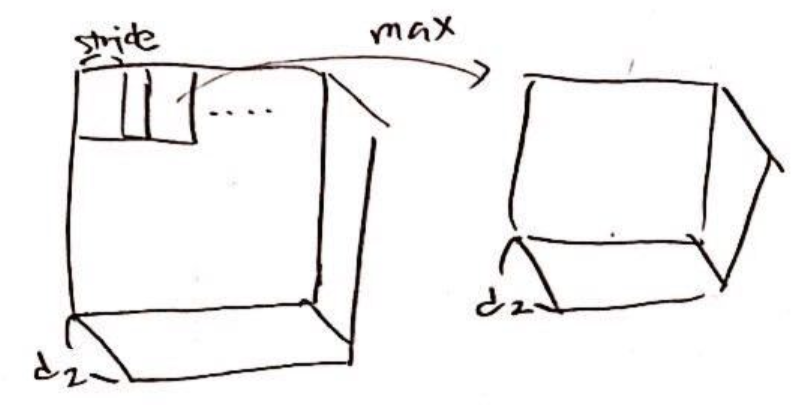
\includegraphics[height=10em]{resources/maxpool2d.png}
}{
  \begin{itemizec}
    \item $|x| = (d_1, d_2, d_3, d_4)\text{ or } (d_2, d_3, d_4)$
    \item $kernel\_size[0] \leq d_3 + 2 \x padding[0]$
    \item $kernel\_size[1] \leq d_4 + 2 \x padding[1]$
  \end{itemizec}
}{
  \begin{itemizec}
    \item $(d_1, d_2, h, w) \text{ or } (d_2, h, w)$ where.. proof tree.
  \end{itemizec}
}{
  \begin{itemizec}
    \item Convolution 다음 activation으로 자주 쓰이는 MaxPool 레이어 입니다.
  \end{itemizec}
}
\begin{align*}
  \frac
  {
    \begin{array}{l}
      \sigma \vdash E \Rar e, c \\
      k = \op{rank}{e} \\
      h_{orig} = e[k-1] \\
      w_{orig} = e[k] \\
      h = \left\lfloor \frac{h_{orig} + 2 \x padding \ind{0} - dilation \ind{0}
        \x (kernel\_size \ind{0} - 1) - 1}{stride \ind{0}} \right\rfloor + 1 \\
      w = \left\lfloor \frac{w_{orig} + 2 \x padding \ind{1} - dilation \ind{1}
        \x (kernel\_size \ind{1} - 1) - 1}{stride \ind{1}} \right\rfloor + 1 \\
      e' = e\indr{1}{k-2} \conc (h, w) \\
      c_{dim} = \{ (k = 3 \lor k = 4) \} \\
      c_w = \{ (kernel\_size\ind{0} \leq h_{orig} + 2 \x padding \ind{0}) \} \\
      c_h = \{ (kernel\_size\ind{1} \leq w_{orig} + 2 \x padding \ind{1}) \} 
    \end{array}
  }
  {
    \begin{array}{c}
      \sigma \vdash \module{MaxPool2d}{kernel\_size, stride=kernel\_size,
        padding=0, dilation=1}{E}
        \Rar e', c \cup c_{dim} \cup c_w \cup c_h 
    \end{array}
  } \\
  \\
  \text{$kernel\_size, stride, padding, dilation$는 가로-세로별 2-tuple로도 들어갈
  수 있음} \\
  \text{이 경우를 위해 $stride\ind{0}, stride\ind{1}$으로 표기함} \\
  \text{만일 $stride$가 튜플이 아닌 스칼라라면 $stride\ind{0}$ 또는 $\ind{1}$은
    $stride$ 값 자체를 의미}
\end{align*}

\prepost{torch.nn.MaxPool2d(kernel\_size, stride=..., dilation=1,
return\_indices=False, ceil\_mode=False)}{
  
\includegraphics[height=8em]{resources/maxpool2d_ri.png}
}{
  \begin{itemizec}
    \item $|x| = (d_1, d_2, d_3, d_4)\text{ or } (d_2, d_3, d_4)$
    \item $kernel\_size[0] \leq d_3 + 2 \x padding[0]$
    \item $kernel\_size[1] \leq d_4 + 2 \x padding[1]$
  \end{itemizec}
}{
  \begin{itemizec}
    \item $(d_1, d_2, h, w) \text{ or } (d_2, h, w)$ where.. proof tree.
    \item $return\_indices$가 $True$이면 인덱스 번호까지 튜플로 반환
    \item $ceil\_mode$가 $True$이면 $floor$대신 $ceil$로 shape 계산
  \end{itemizec}
}
\begin{align*}
  \frac
  {
    \begin{array}{l}
      \sigma \vdash E \Rar e, c \\
      k = \op{rank}{e} \\
      h_{orig} = e[k-1] \\
      w_{orig} = e[k] \\
      h = \left\lfloor \frac{h_{orig} + 2 \x padding \ind{0} - dilation \ind{0}
        \x (kernel\_size \ind{0} - 1) - 1}{stride \ind{0}} \right\rfloor + 1 \\
      w = \left\lfloor \frac{w_{orig} + 2 \x padding \ind{1} - dilation \ind{1}
        \x (kernel\_size \ind{1} - 1) - 1}{stride \ind{1}} \right\rfloor + 1 \\
      h_{ceil} = \left\lceil \frac{h_{orig} + 2 \x padding \ind{0} - dilation \ind{0}
        \x (kernel\_size \ind{0} - 1) - 1}{stride \ind{0}} \right\rceil + 1 \\
      w_{ceil} = \left\lceil \frac{w_{orig} + 2 \x padding \ind{1} - dilation \ind{1}
        \x (kernel\_size \ind{1} - 1) - 1}{stride \ind{1}} \right\rceil + 1 \\
      e' = \ifs{ceil\_mode}{e\indr{1}{k-2} \conc (h_{ceil},
      w_{ceil})}{e\indr{1}{k-2} \conc (h, w)} \\
      e_{out} = \ifs{return\_indices}{(e', e')}{e'}\\
      c_{dim} = \{ (k = 3 \lor k = 4) \} \\
      c_w = \{ (kernel\_size\ind{0} \leq e[3] + 2 \x padding \ind{0}) \} \\
      c_h = \{ (kernel\_size\ind{1} \leq e[4] + 2 \x padding \ind{1}) \} 
    \end{array}
  }
  {
    \begin{array}{rl}
      \sigma \vdash & \module{MaxPool2d}{kernel\_size, stride, padding,
        dilation, return\_indices, ceil\_mode}{E} \\
      & \Rar e', c \cup c_{dim} \cup c_w \cup c_h 
    \end{array}
  } \\
  \\
  \text{$return\_indices$가 $True$이면 (결과, 인덱스) 튜플 형태로 반환}\\
  \text{$ceil\_mode$가 $True$이면 $floor$대신 $ceil$함수로 계산}
\end{align*}

\begin{align*}
  \frac
  {
    \begin{array}{l}
      \sigma \vdash \op{torch.nn.MaxPool2d}{E, other\_params...} \Rar e, c \\
    \end{array}
  }
  {
    \sigma \vdash \op{max\_pool2d}{E, other\_params...} \Rar e, c
  } \\
  \\
  \text{(Builtins) \ttt{torch.max\_pool2d}나
  \ttt{torch.nn.functional.max\_pool2d}에 대한 적용}
\end{align*}%}}}

\section*{Normalizations}
\subsection*{\texttt{torch.nn.BatchNorm2d}}%{{{
\prepost{torch.nn.BatchNorm2d(num\_features, other\_params...)(x)}{
  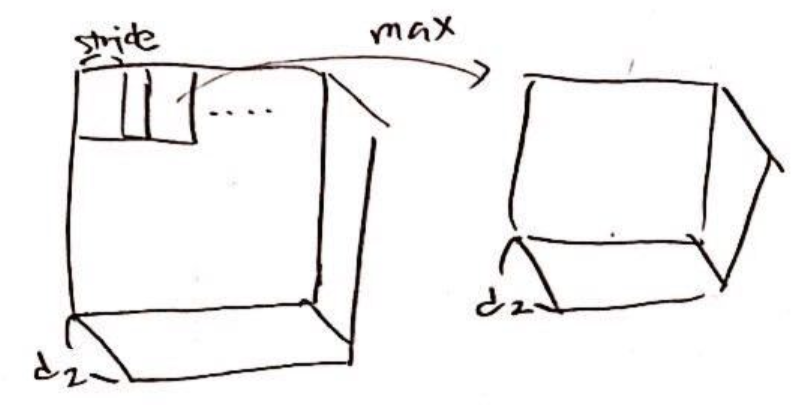
\includegraphics[height=10em]{resources/maxpool2d.png}
}{
  \begin{itemizec}
    \item $|x| = (d_1, d_2, d_3, d_4)$\bigspace ($\mtt{rank} = 4$)
    \item $d_2 = num\_features$
  \end{itemizec}
}{
  \begin{itemizec}
    \item $|y| = (d_1, d_2, d_3, d_4)$\bigspace (same shape to $x$)
  \end{itemizec}
}
\begin{align*}
  \frac
  {
    \begin{array}{l}
      \sigma \vdash E \Rar e, c \\
      c' = \{ (\op{rank}{e} = 4) \land (e[2] = num\_features) \}
    \end{array}
  }
  {
    \sigma \vdash \module{BatchNorm2d}{num\_features, other\_params}{E} \Rar e,
      c \cup c'
  }
\end{align*}
%}}}


\end{document}
